\subsection{Sheaf associated with a presheaf}

Keeping the notation of no. 5, one calls \(\widetilde{\mathcal{F}}\) the sheaf associated with the presheaf \(\mathcal{F}\) , and denotes by \(\widetilde{\mathcal{F}}\) the sheaf \(\underline{\mathcal{L}}(\mathrm{B};\mathrm{E}_{\mathcal{F}})\) the sheaf of continuous sections of the étale B-space \(\mathrm{E}_{\mathcal{F}}\) associated with the presheaf \(\mathcal{F}\) . For every open set \(\mathrm{U}\in\mathcal{B}\) , denote by \(\sigma_{\mathcal{F}}(\mathrm{U})\colon\mathcal{F}(\mathrm{U})\to\widetilde{\mathcal{F}}(\mathrm{U})\) the map which, to \(s\in\mathcal{F}(\mathrm{U})\) , associates the continuous section \(\sigma_{\mathcal{F}}(\mathrm{U},s)\colon x\mapsto[\mathrm{U},s,x]\) of \(\mathrm{E}_{\mathcal{F}}\) over U. By definition of the equivalence relation \(\mathrm{R}_{\mathcal{F}}\) , the family \(\sigma_{\mathcal{F}}=(\sigma_{\mathcal{F}}(\mathrm{U}))_{\mathrm{U}\in\mathcal{B}}\) is a morphism of presheaves from \(\mathcal{F}\) into the presheaf \(\widetilde{\mathcal{F}}|\mathcal{B}\) . The morphism \(\sigma_{\mathcal{F}}\) is called the canonical morphism from \(\mathcal{F}\) into \(\widetilde{\mathcal{F}}|\mathcal{B}\) .

Denote by \(j_{\mathcal{F}} \colon \mathrm{E}_{\mathcal{F}} \to \mathrm{E}_{\widetilde{\mathcal{F}}}\) the B-morphism composed of the canonical B-isomorphism \(\mathrm{E}_{\widetilde{\mathcal{F}}|\mathcal{B}} \to \mathrm{E}_{\widetilde{\mathcal{F}}}\) (I, p.~51) and of the B-morphism \(\mathrm{E}(\sigma_{\mathcal{F}}) \colon \mathrm{E}_{\mathcal{F}} \to \mathrm{E}_{\widetilde{\mathcal{F}}|\mathcal{B}}\). Let us also denote by \(e_{\mathcal{F}} \colon \mathrm{E}_{\widetilde{\mathcal{F}}} \to \mathrm{E}_{\mathcal{F}}\) the canonical B-isomorphism (I, p.~52, example 2).

PROPOSITION 2. --- The map \(j_{\mathcal{F}}\) is the inverse B-isomorphism of \(e_{\mathcal{F}}\) .

For \(\mathrm{U}\in \mathcal{B}\) , \(s\in \mathcal{F}(\mathrm{U})\) and \(x\in \mathrm{U}\) , we have by definition of \(j_{\mathcal{F}}\) :

\[
j _ {\mathcal {F}} ([ \mathrm{U}, s, x ]) = [ \mathrm{U}, \sigma_ {\mathcal {F}} (\mathrm{U}, s), x ],
\]

whence \(e_{\mathcal{F}}(j_{\mathcal{F}}([U,s,x])) = \sigma_{\mathcal{F}}(U,s)(x) = [U,s,x]\). This proves the proposition.

COROLLARY. --- For every \(a \in B\) , the map \((\sigma_{\mathcal{F}})_{a}\) : \(F_{a} \to \widetilde{F}_{a}\) is bijective.

Since \(j_{F}\) is a B-isomorphism, the same is true of \(\mathrm{E}(\sigma_{\mathcal{F}})\) , and \((\sigma_{\mathcal{F}})_{a}\) is obtained by passing to fibers at a.

Let \(\mathcal{G}\) be a presheaf on B relative to \(\mathcal{B}\) and \(\varphi\colon\mathcal{F}\to\mathcal{G}\) a morphism of presheaves. We denote by \(\widetilde{\varphi}\colon\widetilde{\mathcal{F}}\to\widetilde{\mathcal{G}}\) the morphism of sheaves \(\underline{\mathcal{L}}_{\mathrm{E}(\varphi)}\) (I, p.~48, example 1), where \(\mathrm{E}(\varphi)\colon\mathrm{E}_{\mathcal{F}}\to\mathrm{E}_{\mathcal{G}}\) is the B-morphism associated with \(\varphi\) . For every open set \(\mathrm{U}\in\mathcal{B}\) and every \(s\in\mathcal{F}(\mathrm{U})\) , we have, by definition,

\[
\widetilde {\varphi} _ {\mathrm{U}} (\sigma_ {\mathcal {F}} (\mathrm{U}, s)) = \mathrm{E} (\varphi) \circ \sigma_ {\mathcal {F}} (\mathrm{U}, s) = \sigma_ {\mathcal {G}} (\mathrm{U}, \varphi_ {\mathrm{U}} (s)).
\]

Thus we have:

\[
\widetilde {\varphi} _ {\mathrm{U}} \circ \sigma_ {\mathcal {F}} (\mathrm{U}) = \sigma_ {\mathcal {G}} (\mathrm{U}) \circ \varphi_ {\mathrm{U}}, \quad \text {   for   every   } \mathrm{U} \in \mathcal {B}.\tag{1}
\]

In other words:

\[
\widetilde {\varphi} \mid \mathcal {B} \circ \sigma_ {\mathcal {F}} = \sigma_ {\mathcal {G}} \circ \varphi .\tag{2}
\]

PROPOSITION 3. --- Let B be a topological space, let \(\mathcal{B}\) be a base of the topology of B, let \(\mathcal{F} = (\mathcal{F}(\mathrm{U}), f_{\mathrm{UV}})\) be a presheaf on B relative to \(\mathcal{B}\) , let \(\widetilde{\mathcal{F}}\) be the associated sheaf and let \(\sigma_{\mathcal{F}}: \mathcal{F} \to \widetilde{\mathcal{F}} \mid \mathcal{B}\) be the canonical morphism. Given a sheaf \(\mathcal{G} = (\mathcal{G}(\mathrm{U}), g_{\mathrm{UV}})\) on B and a morphism of presheaves \(\varphi: \mathcal{F} \to \mathcal{G} \mid \mathcal{B}\) , there exists a unique morphism of sheaves \(\psi: \widetilde{\mathcal{F}} \to \mathcal{G}\) such that \(\psi \mid \mathcal{B} \circ \sigma_{\mathcal{F}} = \varphi\) .

Lemma. --- Let U be an open subset of B and \(s\colon U \to E_{\mathcal{F}}\) be a continuous section of \(E_{\mathcal{F}}\) above U. For every point a of U, there exists an open set \(V \in \mathcal{B}\) such that \(a \in V\) and \(V \subset U\) and an element v of \(\mathcal{F}(V)\) such that \(s \mid V = \sigma_{\mathcal{F}}(V, v)\) .

Let \(a \in \mathrm{U}\) . By definition of the space \(\mathrm{E}_{\mathcal{F}}\) , there exists an open set \(\mathrm{V}' \in \mathcal{B}\) such that \(a \in \mathrm{V}'\) and an element \(t\) of \(\mathcal{F}(\mathrm{V}')\) such that \(s(a) = [\mathrm{V}', t, a]\) . Then \(s\) and \(\sigma_{\mathcal{F}}(\mathrm{V}', t)\) induce, by restriction, two continuous sections of \(\mathrm{E}_{\mathcal{F}}\) over \(\mathrm{V}' \cap \mathrm{U}\) which are equal at the point \(a\) . By prop. 11, b) of I, p.~34, there exists an open neighborhood V of \(a\) , contained in \(\mathrm{V}' \cap \mathrm{U}\) and belonging to \(\mathcal{B}\) , such that \(s\) and \(\sigma_{\mathcal{F}}(\mathrm{V}', t)\) coincide at every point of V. If one sets \(v = f_{\mathrm{VV}'}(t)\) , one indeed has \(s \mid \mathrm{V} = \sigma_{\mathcal{F}}(\mathrm{V}, v)\) .

Let us prove the proposition. For every open set U of B and every section \(s \in \widetilde{\mathcal{F}}(\mathrm{U})\) , denote by \(\mathrm{D}(\mathrm{U}, s)\) the set of pairs \((\mathrm{V}, v)\) such that \(V \in \mathcal{B}\) , \(V \subset U\) , \(v \in \mathcal{F}(\mathrm{V})\) and \(s | V = \sigma_{\mathcal{F}}(V, v)\). It follows from the lemma that these open sets V form a covering of U.

If there exists a morphism \(\psi\colon\mathcal{F}\to\mathcal{G}\) such that \(\psi\mid\mathcal{B}\circ\sigma_{\mathcal{F}}=\varphi\) , then, for every open set U of B, every section \(s\in\widetilde{\mathcal{F}}(\mathrm{U})\) and every pair \((\mathrm{V},v)\in\mathrm{D}(\mathrm{U},s)\) , we have \(g_{\mathrm{VU}}(\psi_{\mathrm{U}}(s))=\psi_{\mathrm{V}}(s\mid\mathrm{V})=\varphi_{\mathrm{V}}(v)\) . This proves the uniqueness of \(\psi\) by virtue of the property \((\mathrm{F}_{1})\) of sheaves.

Let U be an open set of B and s an element of \(\widetilde{\mathcal{F}}(\mathrm{U})\) . Let \((\mathrm{V},v)\) and \((\mathrm{V}^{\prime},v^{\prime})\) be elements of \(\mathrm{D}(\mathrm{U},s)\) . We have \(s(a)=[\mathrm{V},v,a]=[\mathrm{V}^{\prime},v^{\prime},a]\) for every point \(a\in V\cap V^{\prime}\) . Therefore, there exists a pair \((\mathrm{W},w)\in\mathrm{D}(\mathrm{V}\cap\mathrm{V}^{\prime},s)\) such that \(a\in W\) and \(f_{\mathrm{WV}}(v)=f_{\mathrm{WV}}(v^{\prime})=w\) . One then has

\[
g _ {\mathrm{W} (\mathrm{V} \cap \mathrm{V} ^ {\prime})} \circ g _ {(\mathrm{V} \cap \mathrm{V} ^ {\prime}) \mathrm{V}} (\varphi_ {\mathrm{V}} (v)) = g _ {\mathrm{WV}} (\varphi_ {\mathrm{V}} (v)) = \varphi_ {\mathrm{W}} (f _ {\mathrm{WV}} (v)) = \varphi_ {\mathrm{W}} (w)
\]

and likewise,

\[
g _ {\mathrm{W} (\mathrm{V} \cap \mathrm{V} ^ {\prime})} \circ g _ {(\mathrm{V} \cap \mathrm{V} ^ {\prime}) \mathrm{V} ^ {\prime}} (\varphi_ {\mathrm{V} ^ {\prime}} (v ^ {\prime})) = \varphi_ {\mathrm{W}} (w),
\]

whence

\[
g _ {\mathrm{W} (\mathrm{V} \cap \mathrm{V} ^ {\prime})} \circ g _ {(\mathrm{V} \cap \mathrm{V} ^ {\prime}) \mathrm{V}} (\varphi_ {\mathrm{V}} (v)) = g _ {\mathrm{W} (\mathrm{V} \cap \mathrm{V} ^ {\prime})} \circ g _ {(\mathrm{V} \cap \mathrm{V} ^ {\prime}) \mathrm{V} ^ {\prime}} (\varphi_ {\mathrm{V} ^ {\prime}} (v ^ {\prime})).
\]

By property (F \(_{1}\) ) of sheaves, we therefore have

\[
g _ {(\mathrm{V} \cap \mathrm{V} ^ {\prime}) \mathrm{V}} (\varphi_ {\mathrm{V}} (v)) = g _ {(\mathrm{V} \cap \mathrm{V} ^ {\prime}) \mathrm{V} ^ {\prime}} (\varphi_ {\mathrm{V} ^ {\prime}} (v ^ {\prime})).
\]

By the properties \((\mathrm{F}_{1})\) and \((\mathrm{F}_{2})\) of sheaves, there exists a unique element \(\psi_{\mathrm{U}}(s) \in \mathcal{G}(\mathrm{U})\) such that:

\[
g _ {\mathrm{VU}} \left(\psi_ {\mathrm{U}} (s)\right) = \varphi_ {\mathrm{V}} (v) \quad \text {   for   every   } (\mathrm{V}, v) \in \mathrm{D} (\mathrm{U}, s).\tag{3}
\]

Let \(\psi_{\mathrm{U}}\colon \widetilde{\mathcal{F}} (\mathrm{U})\to \mathcal{G}(\mathrm{U})\) be the map thus defined. It follows immediately from (3) that the family \(\psi = (\psi_{\mathrm{U}})\) is a morphism of sheaves and that we have \(\varphi_{\mathrm{V}} = \psi_{\mathrm{V}}\circ \sigma_{\mathcal{F}}(\mathrm{V})\) for all \(\mathrm{V}\in \mathcal{B}\) .

COROLLARY 1. --- Let B be a topological space, \(\mathcal{F}\) a presheaf on B, \(\widetilde{\mathcal{F}}\) the associated sheaf and \(\sigma_{\mathcal{F}}\colon \mathcal{F} \to \widetilde{\mathcal{F}}\) the canonical morphism. For \(\mathcal{F}\) to be a sheaf, it is necessary and sufficient that \(\sigma_{\mathcal{F}}\) is an isomorphism.

If \(\sigma_{\mathcal{F}}\) is an isomorphism, \(\mathcal{F}\) is a sheaf. Conversely, if \(\mathcal{F}\) is a sheaf, there exists by Proposition 3 a morphism \(\varphi: \widetilde{\mathcal{F}} \to \mathcal{F}\) such that \(\varphi \circ \sigma_{\mathcal{F}} = \operatorname{Id}_{\mathcal{F}}\) . Since \(\operatorname{Id}_{\widetilde{\mathcal{F}}}\) is the unique morphism \(\psi: \widetilde{\mathcal{F}} \to \widetilde{\mathcal{F}}\) such that \(\psi \circ \sigma_{\mathcal{F}} = \sigma_{\mathcal{F}}\) , we then have \(\sigma_{\mathcal{F}} \circ \varphi = \operatorname{Id}_{\widetilde{\mathcal{F}}}\) .

Remark. --- Let B be a topological space, \(\mathcal{F}\) a presheaf on B, \(\mathcal{G}\) a sheaf on B, and \(\varphi\colon\mathcal{F}\to\mathcal{G}\) a morphism of presheaves. The canonical morphism \(\sigma_{\mathcal{G}}\colon\mathcal{G}\to\widetilde{\mathcal{G}}\) is an isomorphism by Corollary 1. By relation (2) of I, p.~54, the unique morphism \(\psi\colon\widetilde{\mathcal{F}}\to\mathcal{G}\) such that \(\psi\circ\sigma_{\mathcal{F}}=\varphi\) therefore is \(\sigma_{\mathcal{G}}^{-1}\circ\widetilde{\varphi}\) .

COROLLARY 2. --- Let B be a topological space, F and G sheaves on B, and φ a morphism of sheaves from F to G. The following assertions are equivalent:

\begin{enumerate}
\def\labelenumi{(\roman{enumi})}
\item
  \(\varphi\) is an isomorphism;
\item
  There exists a basis \(\mathcal{B}\) of the topology of B such that for every \(\mathrm{U} \in \mathcal{B}\) , the map \(\varphi_{\mathrm{U}}\) is bijective;
\item
  For every point \(a\) of B, the map \(\varphi_{a}\) is a bijection from the stalk \(\mathcal{F}_{a}\) onto the stalk \(\mathcal{G}_{a}\) .
\end{enumerate}

The implication (i)⇒(ii) is immediate.

(ii)⇒(iii): consider the commutative diagram (I, p.~51)

\[
\begin{array}{c} \mathrm{E} _ {\mathcal {F} | \mathcal {B}} \xrightarrow {\mathrm{E} (\varphi | \mathcal {B})} \mathrm{E} _ {\mathcal {G} | \mathcal {B}} \\ \Big \downarrow \qquad \qquad \qquad \qquad \qquad \Big \downarrow \\ \mathrm{E} _ {\mathcal {F}} \xrightarrow {\mathrm{E} (\varphi)} \mathrm{E} _ {\mathcal {G}}, \end{array}
\]

where the vertical arrows are the canonical B-isomorphisms. If condition (ii) is satisfied, \(\mathrm{E}(\varphi \mid \mathcal{B})\) is a B-isomorphism, hence \(\mathrm{E}(\varphi)\) is one as well. The maps \(\varphi_{a}\) are deduced from \(\mathrm{E}(\varphi)\) by passing to the fibers and are then bijective.

(iii)⇒(i): under hypothesis (iii), the map \(\mathrm{E}(\varphi)\colon E_{\mathcal{F}} \to E_{\mathcal{G}}\) is a bijective B-morphism of étale spaces, hence is a B-isomorphism (I, p.~30, cor. 2 of prop. 6). Consequently, the morphism \(\widetilde{\mathcal{F}}\to\widetilde{\mathcal{G}}\) is an isomorphism. Since \(\mathcal{F}\) and \(\mathcal{G}\) are sheaves, the canonical morphisms \(\sigma_{\mathcal{F}}\colon\mathcal{F}\to\widetilde{\mathcal{F}}\) and \(\sigma_{\mathcal{G}}\colon\mathcal{G}\to\widetilde{\mathcal{G}}\) are isomorphisms (corollary 1), and one has \(\widetilde{\varphi}\circ\sigma_{\mathcal{F}}=\sigma_{\mathcal{G}}\circ\varphi\) (I, p.~54, relation (2)); therefore \(\varphi\) is an isomorphism.

Scholium. --- Let B be a topological space. To every sheaf \(\mathcal{F}\) on B, one associates an étale B-space \(\mathrm{E}_{\mathcal{F}}\) (I, p.~50, def. 4). To every étale B-space T, one associates the sheaf \(\underline{\mathcal{L}}(\mathrm{T})\) on B of its continuous sections (I, p.~45, example 3). There is a canonical isomorphism of sheaves \(\sigma_{\mathcal{F}}\colon \mathcal{F}\to \underline{\mathcal{L}}(\mathrm{E}_{\mathcal{F}})\) (I, p.~55, cor. 1) and a canonical isomorphism of étale B-spaces \(e_{\mathrm{T}}\colon \mathrm{E}_{\underline{\mathcal{L}}(\mathrm{T})}\to \mathrm{T}\) (I, p.~52, example 2).

For every pair \((\mathcal{F},\mathcal{G})\) of sheaves on B, one has defined (I, p.~50) a map \(\varphi\mapsto\mathrm{E}(\varphi)\) of the set of sheaf morphisms from \(\mathcal{F}\) to \(\mathcal{G}\) into the set of B-morphisms from \(E_{F}\) into \(E_{G}\) . We have the relations

\[
\mathrm{E} (\mathrm{Id} _ {\mathcal {F}}) = \mathrm{Id} _ {\mathrm{E} _ {\mathcal {F}}}, \qquad \mathrm{E} (\psi \circ \varphi) = \mathrm{E} (\psi) \circ \mathrm{E} (\varphi).
\]

For every pair (T, U) of étale B-spaces, a map was defined (I, p.~48, example 1) \(f \mapsto \underline{\mathcal{L}}(f)\) of the set of B-morphisms from T to U into the set of sheaf morphisms from \(\underline{\mathcal{L}}(T)\) into \(\underline{\mathcal{L}}(U)\) . We have the relations

\[
\underline {{\mathcal {S}}} (\mathrm{Id} _ {\mathrm{T}}) = \mathrm{Id} _ {\underline {{\mathcal {S}}} (\mathrm{T})}, \qquad \underline {{\mathcal {S}}} (g \circ f) = \underline {{\mathcal {S}}} (g) \circ \underline {{\mathcal {S}}} (f).
\]

With the previous notation, the following diagrams are commutative:

\begin{enumerate}
\def\labelenumi{(\arabic{enumi})}
\setcounter{enumi}{3}
\tightlist
\item
\item
  \pandocbounded{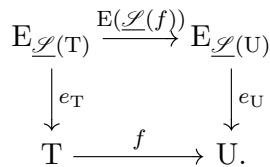
\includegraphics[keepaspectratio]{images/part001_16180f76.jpg}}
\end{enumerate}

This follows from I, p.~54, formula (2) for the first, and it is an immediate consequence of the definitions for the second. This implies that for every pair \((\mathcal{F},\mathcal{G})\) of sheaves on B and every pair (T,U) of étale B-spaces, the maps \(\varphi\mapsto\mathrm{E}(\varphi)\) and \(f\mapsto\underline{\mathcal{L}}(f)\) considered above are bijective.

These results make it possible to deduce a statement about étale B-spaces from a statement about sheaves on B, and conversely.

